% THIS IS SIGPROC-SP.TEX - VERSION 3.1
% WORKS WITH V3.2SP OF ACM_PROC_ARTICLE-SP.CLS
% APRIL 2009
%
% It is an example file showing how to use the 'acm_proc_article-sp.cls' V3.2SP
% LaTeX2e document class file for Conference Proceedings submissions.
% ----------------------------------------------------------------------------------------------------------------
% This .tex file (and associated .cls V3.2SP) *DOES NOT* produce:
%       1) The Permission Statement
%       2) The Conference (location) Info information
%       3) The Copyright Line with ACM data
%       4) Page numbering
% ---------------------------------------------------------------------------------------------------------------
% It is an example which *does* use the .bib file (from which the .bbl file
% is produced).
% REMEMBER HOWEVER: After having produced the .bbl file,
% and prior to final submission,
% you need to 'insert'  your .bbl file into your source .tex file so as to provide
% ONE 'self-contained' source file.
%
% Questions regarding SIGS should be sent to
% Adrienne Griscti ---> griscti@acm.org
%
% Questions/suggestions regarding the guidelines, .tex and .cls files, etc. to
% Gerald Murray ---> murray@hq.acm.org
%
% For tracking purposes - this is V3.1SP - APRIL 2009

\documentclass{acm_proc_article-sp}

\usepackage[hidelinks]{hyperref}
\usepackage{float}
\usepackage{subcaption}
\usepackage{placeins}
\usepackage{needspace}

\usepackage{listings}
\newcommand{\includecode}[2][C]{
    \lstinputlisting[breakatwhitespace=true, breaklines=true,
        basicstyle=\footnotesize, showstringspaces=false, 
        literate={"}{\textquotedbl}1, numbers=left, 
        language=#1]{#2}}

\floatstyle{boxed}
\newfloat{listing}{thp}{lop}
\floatname{listing}{Listing}

\begin{document}

\title{Specialization Annotated OpenCL}

\numberofauthors{1}
\author{
\alignauthor
Nat Tuck\\
       \affaddr{University of Massachusetts Lowell}\\
       \affaddr{One University Avenue}\\
       \affaddr{Lowell, MA}\\
       \email{ntuck@cs.uml.edu}
}

\date{28 August 2014}

\maketitle

\begin{abstract} 
    
This paper describes Specialization Annotated OpenCL, an extension of the
OpenCL parallel programming standard that enables just in time value
specialization. This extension allows some arguments to an OpenCL kernel to be
marked for specialization. Compilation is then delayed until concrete argument
values are available, at which point specialized versions of the kernel are
generated and executed. 

Value specialization, replacing a variable in a program with a known constant
for a particular data set, is an optimization that is commonly performed by
hand for HPC kernels. This optimization cannot be performed automatically in a
programming environment using ahead-of-time compilation, because the input data
is not available to the compiler. With OpenCL, kernel compilation is performed
just-in-time as the program runs.

We have built two implementations of Specialization Annotated OpenCL. The first
is based on the open source POCL library, an open source implementation of
OpenCL built on LLVM that can execute kernels on multi-core CPUs. The second
implementation is a library called Pancake that can be used with unmodified
OpenCL runtimes and allows Specialization Annotated OpenGL to be used on
graphics processors. 

Both implementations are described and performance benchmarks are provided
for each on eight test cases.

\end{abstract}

% A category with the (minimum) three required fields
\category{D.3.4}{Programming Languages}{Processors}[Compilers, Optimization,
Just-In-Time]

\terms{Performance}

\needspace{5\baselineskip}
\section{Introduction}

When implementing an algorithm for an HPC application, it is a common practice
to embed specific values used in the computation in the program source rather
than passing them in as parameters. For example, a program that simulated the
weather on a 500 meter grid may have the literal value ``500'' hard coded as a
global constant used throughout the program.

This technique has both advantages and drawbacks. From a software design
perspective, the drawbacks are most obvious: hard coding a value makes changing
the value more difficult than if the value were passed as a parameter. Further,
it means that the code must be duplicated if the algorithm is used with two
different values in the same program execution. 

The advantage to hard-coding values is that the program will tend to run faster.
Compilers can do several optimizations with constant values that don't work as
well with variables, including arithmetic simplification and loop unrolling.

This technique is called value specialization. When a compiler does it, it is
sometimes called partial evaluation \cite{Futamura:1971:PE}.

If the set of values to be specialized on is known when the program is written,
this problem can be easily solved using techniques like C++ templates.
Templates perform specialization, and they can be parameterized with values to
perform value specialization. But this still produces a program that only works
on some specific set of predecided input values.

It would be nice if the compiler could perform this optimization automatically
for values passed in to the program at run-time. In order to do that, the compiler
would need to execute while the program was running.

OpenCL, the cross-platform parallel programming standard developed for GPU
programming, compiles compute kernels just-in-time as the program runs. We have
developed an extension to OpenCL, Specialization Annotated OpenCL, that allows
this optimization to be performed either by the compiler or by a library linked
in to an OpenCL program. Implementations using these two techniques are
described in Section~\ref{pocl-spec} and Section~\ref{pancake-spec}
respectively.

\needspace{5\baselineskip}
\section{Related Work}

Both specialization and JIT compilation are common techniques used in compiler
systems. Just in time specialization on types is an essential technique for
efficiently executing dynamic languages, described in detail by Chambers in his
dissertation on the Self system \cite{Chambers:1992:Self}.

Just in time value specialization is less common, but is still used in a
variety of existing systems. For example, Apple uses LLVM to specialize shaders
on their Mac OS X implementation of OpenGL. According to a mailing list post by
Chris
Lattner\footnote{\url{http://lists.cs.uiuc.edu/pipermail/llvmdev/2006-August/006492.html}},

\begin{quote}
[Apple's OpenGL implementation does] runtime code specialization within the
fixed-function vertex-processing pipeline. Basically, the OpenGL pipeline has
many parameters (is fog enabled?  do vertices have texture info? etc) which
rarely change: executing the fully branchy code swamps the branch predictors
and performs poorly. To solve this, the code is precompiled to LLVM .bc form,
from which specializations of the code are made, optimized, and JIT compiled as
they are needed at runtime.
\end{quote}

The POCL OpenCL runtime, which our implementation of Specialization Annotated
OpenCL is built on, already specializes kernels on work group
size\footnote{\url{http://pocl.sourceforge.net/docs/html/kernel\_compiler.html}}.
POCL runs each work group in its own thread, and processes the items in a work
group by looping through them. Specializing on workgroup size means that the
number of work items per thread (and thus the size of the loop) is a known
constant. This simplifies the correct implementation of the OpenCL
specification by allowing easier static analysis and transformation of this
work-item loop, which is necessary to implement OpenCL's barrier semantics in
POCL's one thread per workgroup model.

\section{Specialization Annotated OpenCL}

Specialization Annotated OpenCL extends OpenCL by adding annotations to mark
some arguments for specialization. Kernels are annotated by adding a specially
formatted comment as shown on the second line of the sample compute kernel in
Listing~\ref{mmul-spec}. This comment comes between the argument list of the
kernel and the opening brace of the body and contains the {\tt @spec} symbol
followed by the name of the kernel and the list of arguments to be specialized
in parentheses.

\begin{listing}
\includecode{mmul-spec.cl}
\caption{mmul.cl: Example specialization annotation}
\label{mmul-spec}
\end{listing}

When a kernel with a specialization annotation is called, a specialized version
of that kernel is generated with the specialized arguments replaced by the values
used in that call. For example, if the kernel in Listing~\ref{mmul-spec} is called
with the values ($nn = mm = 8$), a specialized kernel is generated that is
functionally equivalent to the code shown in Listing~\ref{mmul-spec-example}.

\begin{listing}
\includecode{mmul-spec-example.cl}
\caption{mmul-codegen.cl: Execution model example}
\label{mmul-spec-example}
\end{listing}

Once the specialized kernel has been generated, it is called with the remaining
(non-specialized) arguments provided in the call. Specialized kernels are
cached for future calls with the same values for the specialized arguments.

We have built two implementations of Specialization Annotated OpenCL,
Specializing POCL and Pancake. These are described in Section~\ref{pocl-spec}
and Section~\ref{pancake-spec} respectively.

\section{Specializing POCL}
\label{pocl-spec}

The first implementation of Specialization Annotated OpenCL described in this
paper is Specializing POCL. This implementation works by modifying the POCL
OpenCL runtime to add support for specialization. 

POCL is an open source implementation of OpenCL supporting execution on
multi-core CPUs and several types of specialized acceleration hardware. It was
initially developed by Pekka Jaaskelainen and others at the Tampere University
of Technology in Finland and the Universidad Rey Juan Calos in Spain in order
to study the design of application specific processor hardware, but has since
been extended for use as a general purpose OpenCL implementation
\cite{Jaaskelainen:2010:POCL}. It is currently the most mature open source
implementation of OpenCL and provides good support for the OpenCL 1.2 standard
on x86\_64 multi-core CPUs.

POCL is built on the LLVM compiler construction toolkit
\cite{Lattner:2002:LLVM}. In broad strokes, POCL uses the Clang C front end to
parse OpenCL C and generate LLVM code, does most of its work in custom LLVM
transformation passes, and then uses an appropriate LLVM back-end to generate
kernel binaries for execution.

In order to extend POCL to support Specialization Annotated OpenCL, three
changes were needed. First, we added code to intercept the OpenCL kernel source
and  extract the specialization annotations. Second, we extracted the values of
the specialized parameters when the kernel was called. Finally, we added an
additional optimization pass during code generation to perform the
specialization.

In order to generate specialized kernels, an LLVM module pass was written.
This optimization pass operates by iterating through the arguments of each
kernel function in the module, seeing if the name matches an argument marked
for specialization in that kernel, and, if so, replacing all uses of that
argument's value with constant value passed to the kernel call. 

The operation of replacing all uses of an argument with a new value is simple.
The LLVM API provides a method ({\tt replaceAllUsesWith}) that does exactly
this. Because LLVM uses an SSA-based intermediate representation, this works
well even if the argument variable is modified during kernel execution, which
would be a problem if specialization was implemented by textual substitution.

Specialization was implemented for 32-bit integers, 64-bit integers, floats,
and doubles. This was sufficient to run the various kernels used for testing the
implementation, but support for other scalar types could be easily added.
Specialization on arrays is an interesting possible extension (consider
specializing an image convolution function on a specific convolution matrix),
but this possibility was not explored.

\section{Performance of Specializing POCL}

In order to test the performance and correctness of our two implementations of
Specialization Annotated OpenCL, eight test cases were selected and benchmarked.
The test cases and comments on their individual performance are detailed in
Section~\ref{test-cases}. 

For Specializing POCL, tests were run on a 24-core workstation with two AMD
Opteron 6234 processors. None of the test cases used enough RAM for that to be
a bottleneck. 

Each test case was run with six different compiler configurations: three
different levels of optimization each with and without specialization enabled.
The three levels of optimization are none (``default''), loop unrolling only
(``unroll''), and the full set of standard LLVM optimizations (``O3'').

The test cases were run five times for each configuration. The results are
shown in Figure~\ref{socl-pocl-table}. The bars show the median measurement,
while the error bars show minimum and maximum measurements. Configurations with
specialization enabled are shown in blue.

% A summary of the best speedups is shown in Table~\ref{cake-speedups-table}.
% % This file is autogenerated.
%
% Edit the source CSVs or the generator script (data2speeups.pl)

\begin{table}
\centering
\begin{tabular}{ l | r | r | r }

\textbf{Benchmark} & \textbf{Spec} & \textbf{Spec + Unroll} & \textbf{Spec + O3} \\

blur & 21.5\% & -23.4\% & -23.0\% \\
mandelbrot & -0.9\% & 0.3\% & -0.6\% \\
mmul & -0.3\% & 122.6\% & -11.0\% \\
nas-cg & -19.6\% & -22.2\% & -21.4\% \\
nas-sp & 193.1\% & 169.5\% & 156.2\% \\
nv-bs & -1.1\% & -1.9\% & -6.6\% \\
nv-dct & -0.0\% & 30.8\% & 36.4\% \\
particlefilter & -4.0\% & -2.7\% & -2.7\% \\
\end{tabular}
\caption{Speedups with Modified POCL}
\label{cake-speedups-table}
\end{table}



Initially, the main driver of performance gains was expected to be loop
unrolling enabled by making the loop trip count constant. This turned out not
to be the case. The Opteron's superscalar architecture is able to handle simple
loops very well through instruction-level parallelism and branch prediction,
which negates the benefit of loop unrolling \cite{Jouppi:1989:ILP}.

Three test cases showed significant speedups, while two showed significant
slowdowns. Two of these tests benefited from specialization for loop unrolling.
Results for each test are described in Section~\ref{test-cases}.

\begin{figure*}
\mbox{\hspace*{0.0\textwidth}
\begin{subfigure}[b]{0.55\textwidth}
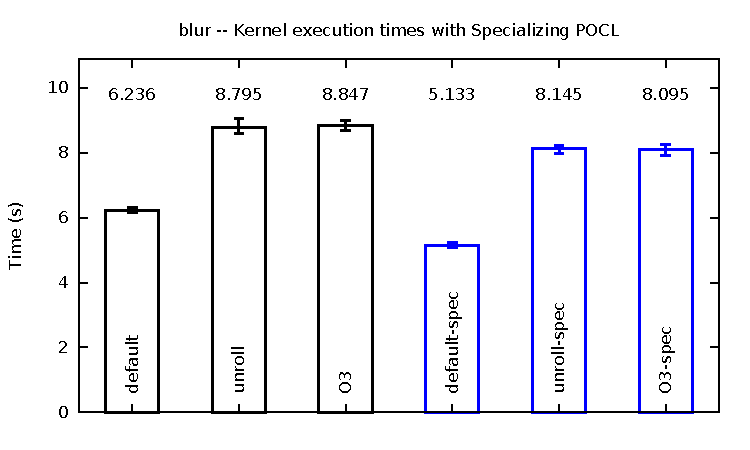
\includegraphics[width=3.0in]{charts/pocl/blur-exec}
\end{subfigure}
\begin{subfigure}[b]{0.55\textwidth}
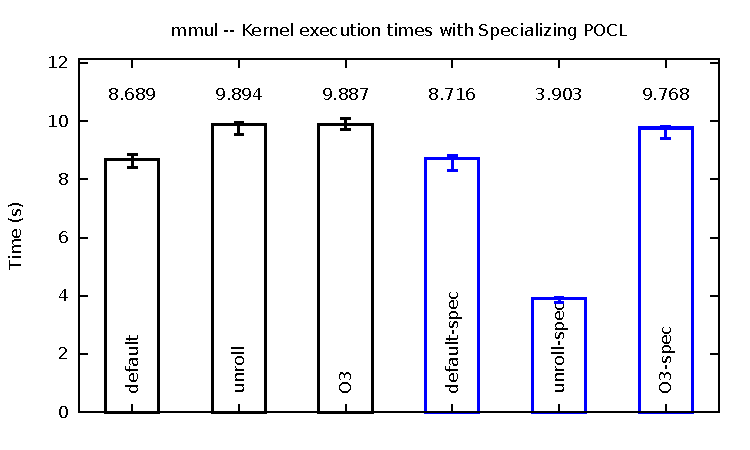
\includegraphics[width=3.0in]{charts/pocl/mmul-exec}
\end{subfigure}}

\mbox{\hspace*{0.0\textwidth}
\begin{subfigure}[b]{0.55\textwidth}
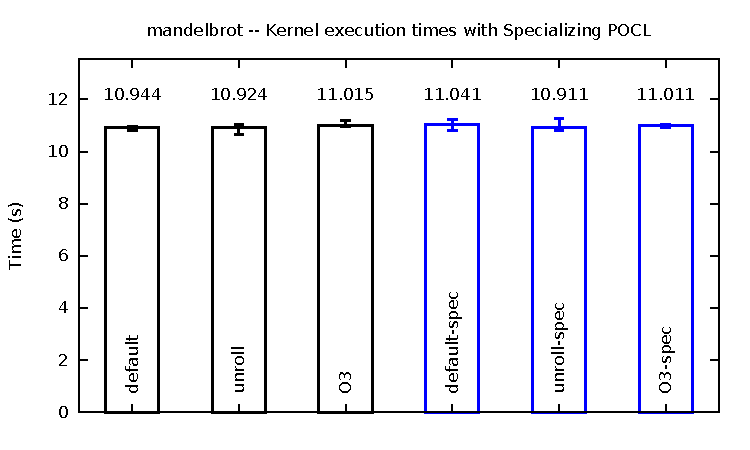
\includegraphics[width=3.0in]{charts/pocl/mandelbrot-exec}
\end{subfigure}
\begin{subfigure}[b]{0.55\textwidth}
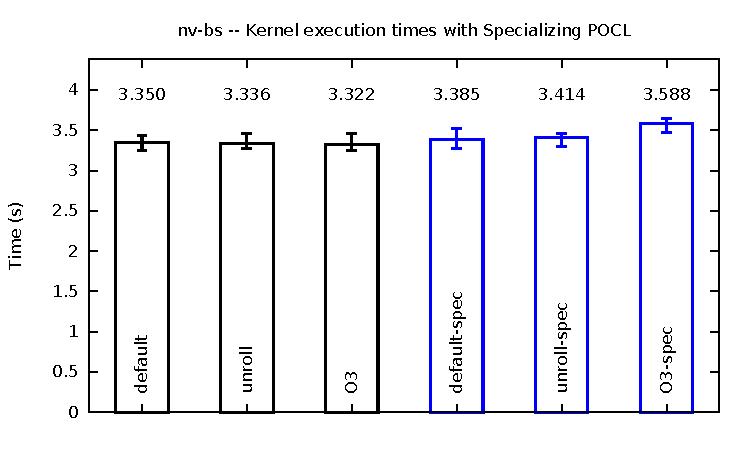
\includegraphics[width=3.0in]{charts/pocl/nv-bs-exec}
\end{subfigure}}

\mbox{\hspace*{0.0\textwidth}
\begin{subfigure}[b]{0.55\textwidth}
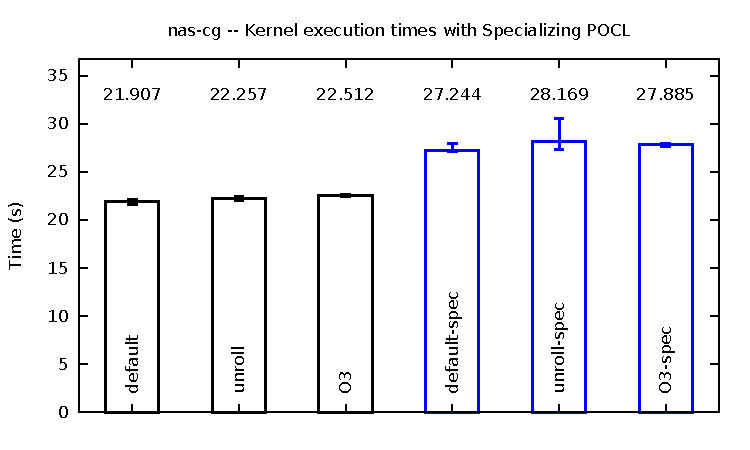
\includegraphics[width=3.0in]{charts/pocl/nas-cg-exec}
\end{subfigure}
\begin{subfigure}[b]{0.55\textwidth}
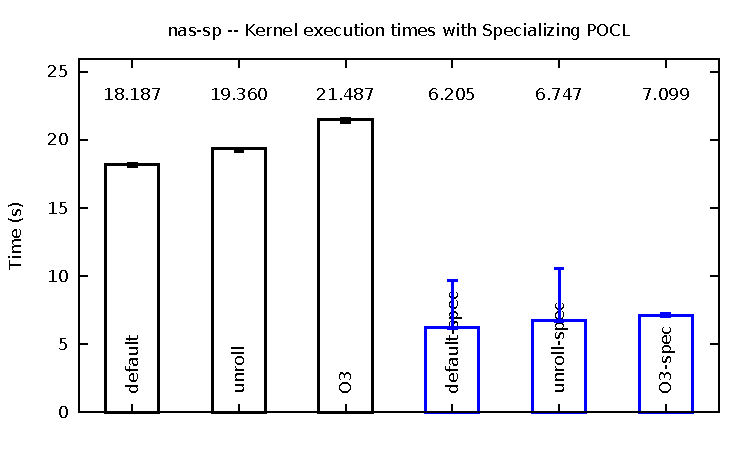
\includegraphics[width=3.0in]{charts/pocl/nas-sp-exec}
\end{subfigure}}

\mbox{\hspace*{0.0\textwidth}
\begin{subfigure}[b]{0.55\textwidth}
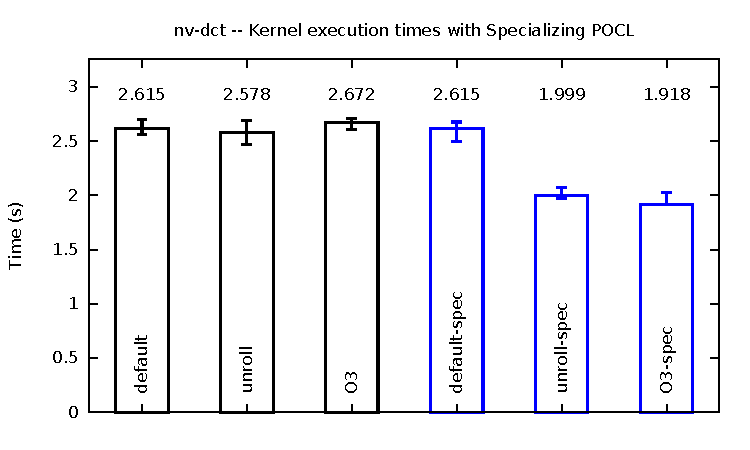
\includegraphics[width=3.0in]{charts/pocl/nv-dct-exec}
\end{subfigure}
\begin{subfigure}[b]{0.55\textwidth}
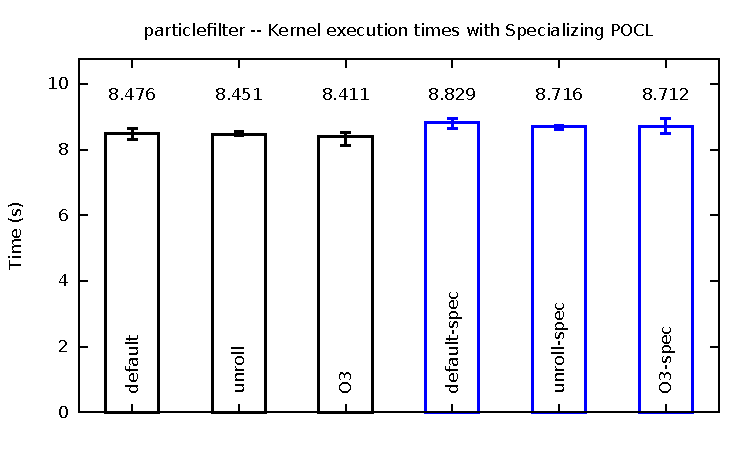
\includegraphics[width=3.0in]{charts/pocl/particlefilter-exec}
\end{subfigure}}

\caption{\label{socl-pocl-table} Benchmark timings for Specializing POCL 
    on 24-Core Workstation}
\end{figure*}




\section{Pancake}
\label{pancake-spec}

Our second implementation is Pancake, a C library that can be added to an
existing OpenCL program, which can then be executed with any OpenCL runtime as
Specialization Annotated OpenCL. Pancake was written to allow performance to be
tested with proprietary implementations of OpenCL, such as the GPU OpenCL
runtimes from AMD and Nvidia.

Pancake operates by intercepting calls to the OpenCL API and generating
specialized OpenCL source code that is then passed on to the underlying OpenCL
library. This requires the inclusion of a C header in each file that uses
OpenCL functions which defines macros to intercept the appropriate API calls.

\section{Performance of Pancake}

Pancake was tested on the eight test cases described in
Section~\ref{test-cases} using the AMD and Nvidia proprietary OpenCL runtimes.
Because the compiler settings in these implementations are less accessible than
for the POCL runtime, each test case was only run under four different compiler
configurations (default, default-spec, default-unroll, and spec-unroll). In
order to enable loop unrolling for the ``unroll'' configurations, Pancake added
``{\tt \#pragma unroll}'' to each loop in its OpenCL output.

Pancake was tested on two different machines, the Opteron workstation mentioned
earlier with a Nvidia GeForce GTX 650 Ti graphics card and a desktop system
with an AMD Radeon 5830 graphics card. On the AMD GPU, five test cases showed
speedups while one showed a small slowdown. On the Nvidia, GPU, four showed
speedups and one showed a small slowdown.

Timings with Pancake are shown in Table~\ref{pancake-amd-table} for the AMD GPU
and Table~\ref{pancake-nvidia-table} for the Nvidia GPU. Configurations with
specialization enabled are shown in blue.

%A summary of the best speedups with
%Pancake is shown in Table~\ref{pancake-speedups-table}.

Overall, the performance benefits of specialization were better with Pancake on
GPU devices compared to specializing POCL on a CPU. Initial testing with
Pancake on the AMD OpenCL implementation for CPUs confirmed that this is most
likely due to the hardware rather than the different implementation strategy
for specialization. 

% % This file is autogenerated.
%
% Edit the source CSVs or the generator script (data2speeups.pl)

\begin{table}
\centering
\begin{tabular}{ l | r | r }

\textbf{Benchmark} & \textbf{AMD R 5830} & \textbf{NV GTX 650 Ti} \\

blur & 175.5\% & 16.1\% \\
mandelbrot & 3.6\% & 23.5\% \\
mmul & 91.4\% & 86.7\% \\
nas-cg & -1.6\% & -0.4\% \\
nas-sp & 0.1\% & 0.2\% \\
nv-bs & 8.0\% & 1.0\% \\
nv-dct & 3.5\% & 2.0\% \\
particlefilter & 0.2\% & -2.7\% \\
\end{tabular}
\caption{Speedups with Pancake}
\label{pancake-speedups-table}
\end{table}




%\newgeometry{left=1.5in,right=1.5in,top=0.20in,bottom=1.0in}

\begin{figure*}

\mbox{\hspace*{0.0\textwidth}
\begin{subfigure}[b]{0.55\textwidth}
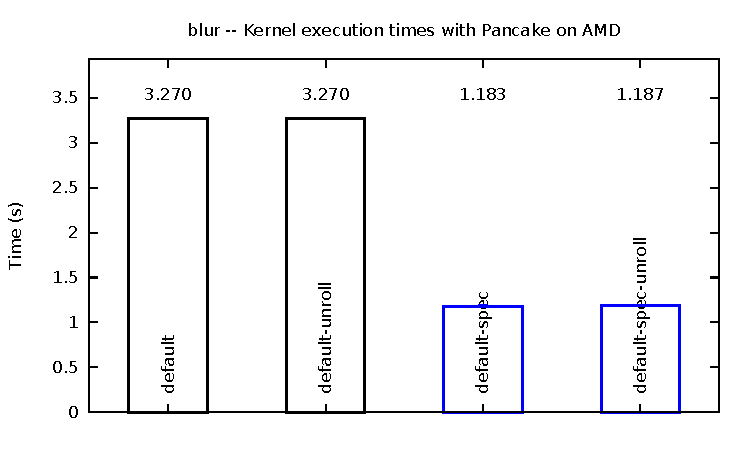
\includegraphics[width=3.0in]{charts/amd/blur-exec}
\end{subfigure}
\begin{subfigure}[b]{0.55\textwidth}
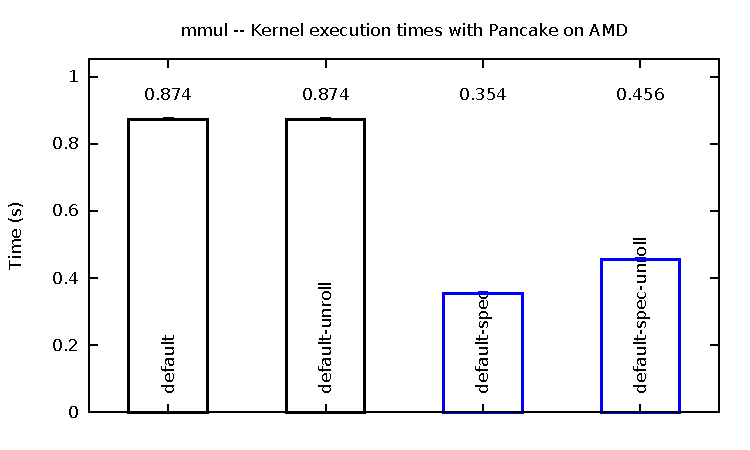
\includegraphics[width=3.0in]{charts/amd/mmul-exec}
\end{subfigure}}

\mbox{\hspace*{0.0\textwidth}
\begin{subfigure}[b]{0.55\textwidth}
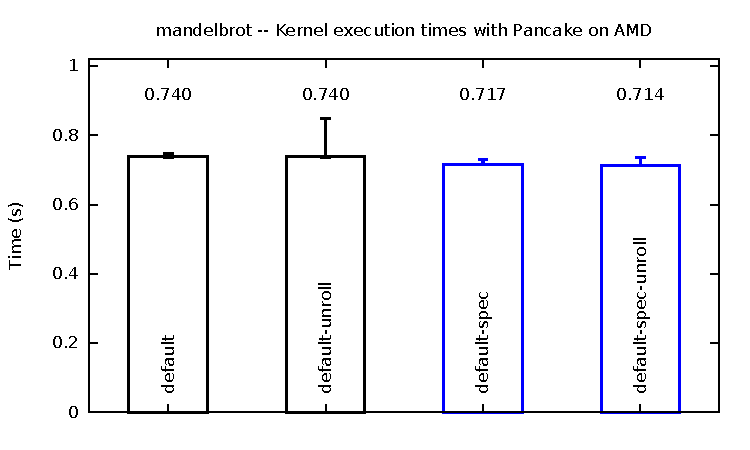
\includegraphics[width=3.0in]{charts/amd/mandelbrot-exec}
\end{subfigure}
\begin{subfigure}[b]{0.55\textwidth}
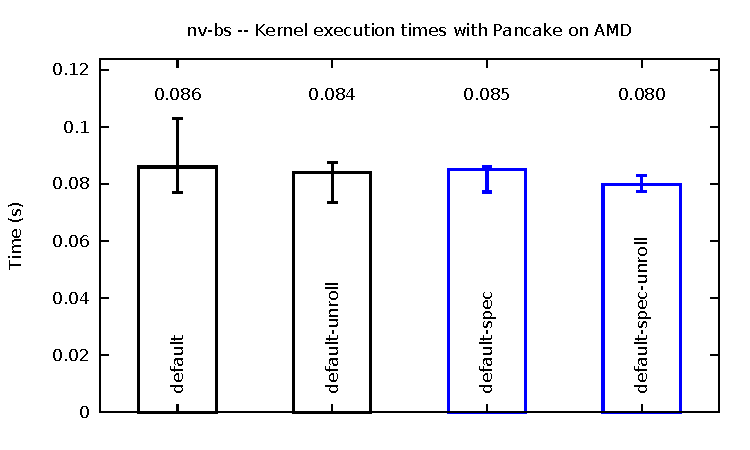
\includegraphics[width=3.0in]{charts/amd/nv-bs-exec}
\end{subfigure}}

\mbox{\hspace*{0.0\textwidth}
\begin{subfigure}[b]{0.55\textwidth}
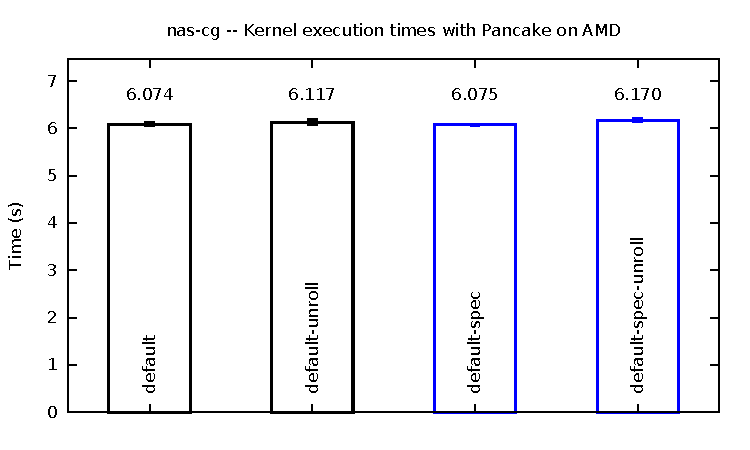
\includegraphics[width=3.0in]{charts/amd/nas-cg-exec}
\end{subfigure}
\begin{subfigure}[b]{0.55\textwidth}
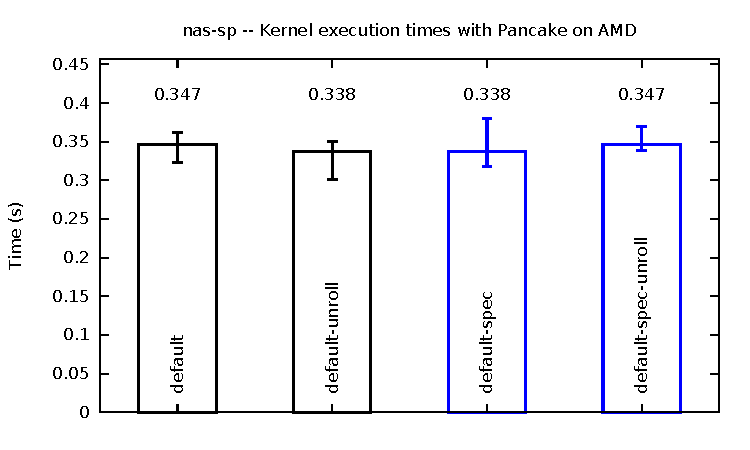
\includegraphics[width=3.0in]{charts/amd/nas-sp-exec}
\end{subfigure}}

\mbox{\hspace*{0.0\textwidth}
\begin{subfigure}[b]{0.55\textwidth}
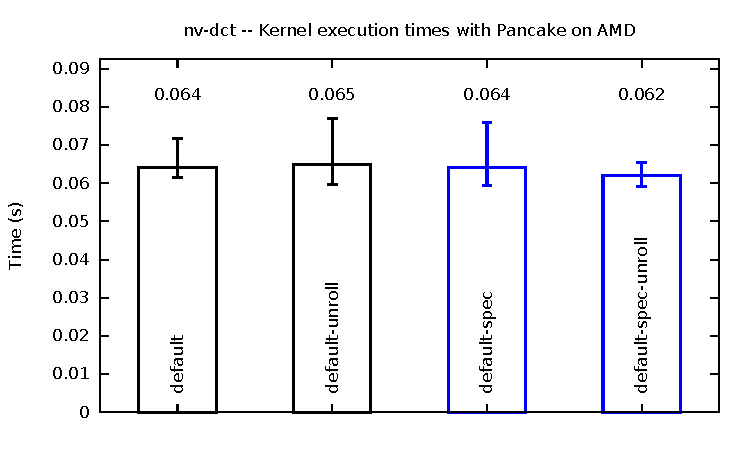
\includegraphics[width=3.0in]{charts/amd/nv-dct-exec}
\end{subfigure}
\begin{subfigure}[b]{0.55\textwidth}
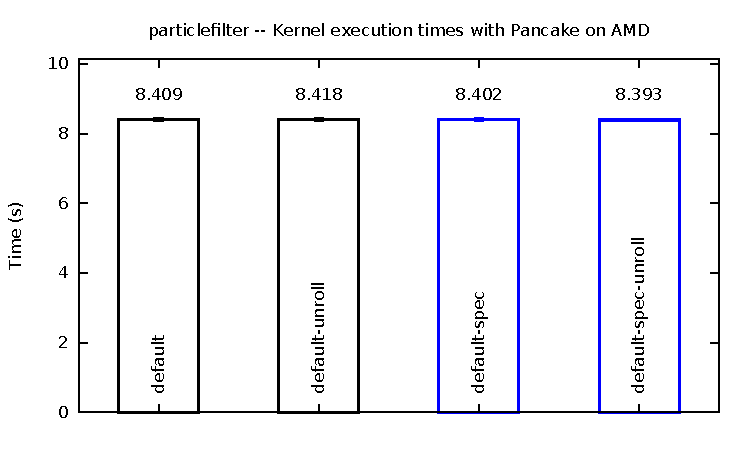
\includegraphics[width=3.0in]{charts/amd/particlefilter-exec}
\end{subfigure}}

\caption{\label{pancake-amd-table} Benchmark Timings for Pancake on AMD Radeon 5830}
\end{figure*}

%\restoregeometry



%\newgeometry{left=1.5in,right=1.5in,top=0.20in,bottom=1.0in}

\begin{figure*}

\mbox{\hspace*{0.0\textwidth}
\begin{subfigure}[b]{0.55\textwidth}
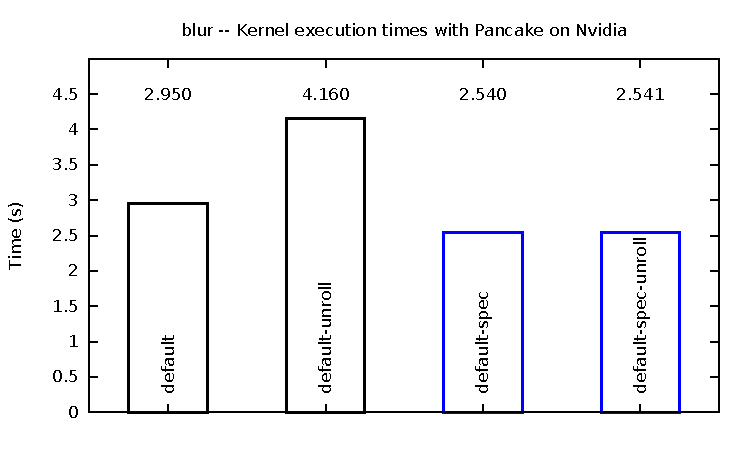
\includegraphics[width=3.0in]{charts/nvidia/blur-exec}
\end{subfigure}
\begin{subfigure}[b]{0.55\textwidth}
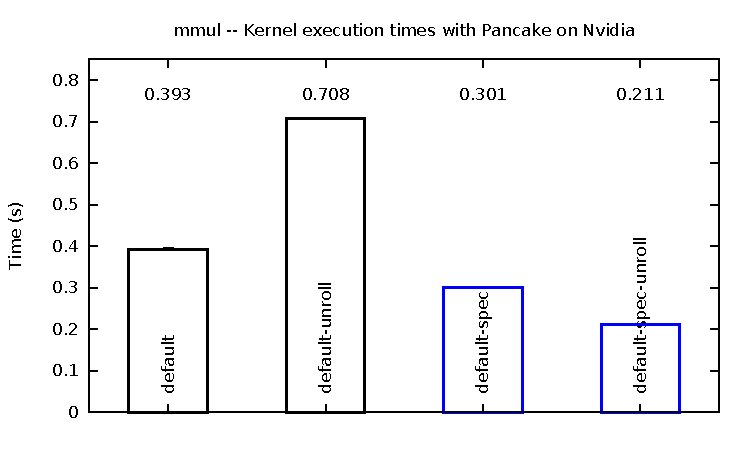
\includegraphics[width=3.0in]{charts/nvidia/mmul-exec}
\end{subfigure}}

\mbox{\hspace*{0.0\textwidth}
\begin{subfigure}[b]{0.55\textwidth}
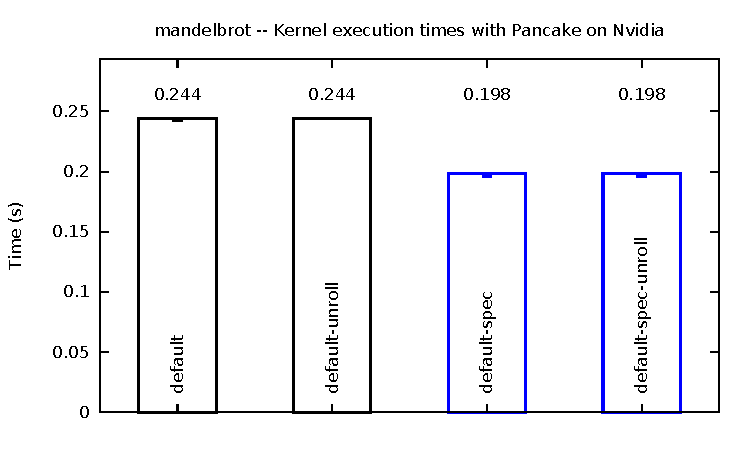
\includegraphics[width=3.0in]{charts/nvidia/mandelbrot-exec}
\end{subfigure}
\begin{subfigure}[b]{0.55\textwidth}
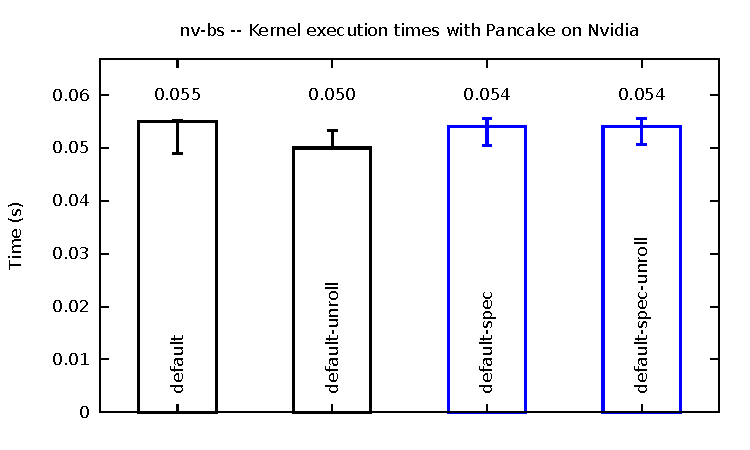
\includegraphics[width=3.0in]{charts/nvidia/nv-bs-exec}
\end{subfigure}}

\mbox{\hspace*{0.0\textwidth}
\begin{subfigure}[b]{0.55\textwidth}
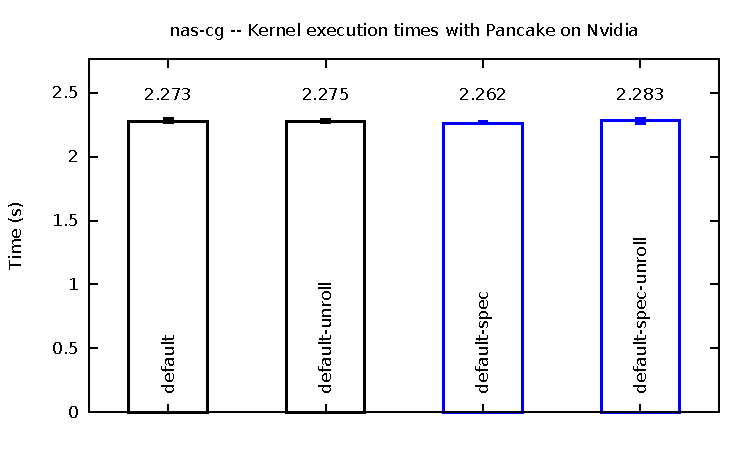
\includegraphics[width=3.0in]{charts/nvidia/nas-cg-exec}
\end{subfigure}
\begin{subfigure}[b]{0.55\textwidth}
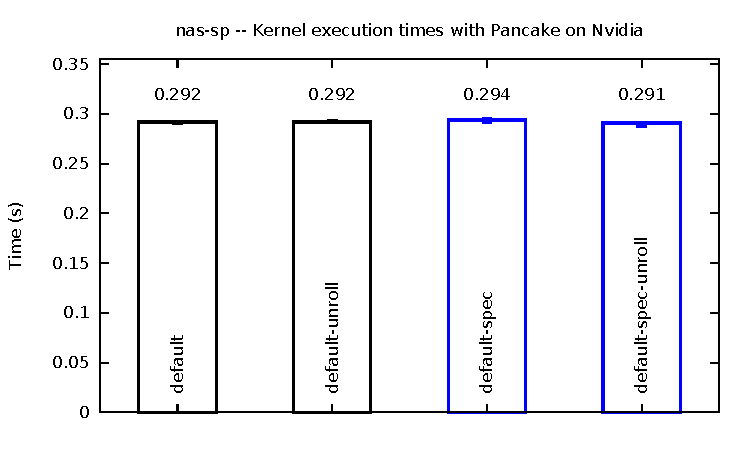
\includegraphics[width=3.0in]{charts/nvidia/nas-sp-exec}
\end{subfigure}}

\mbox{\hspace*{0.0\textwidth}
\begin{subfigure}[b]{0.55\textwidth}
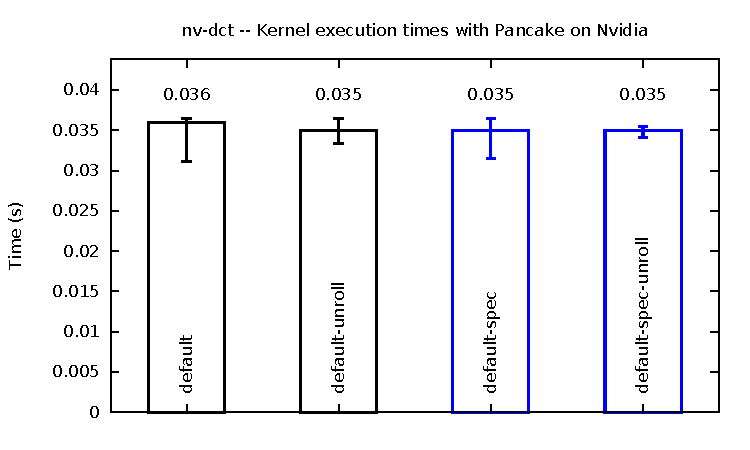
\includegraphics[width=3.0in]{charts/nvidia/nv-dct-exec}
\end{subfigure}
\begin{subfigure}[b]{0.55\textwidth}
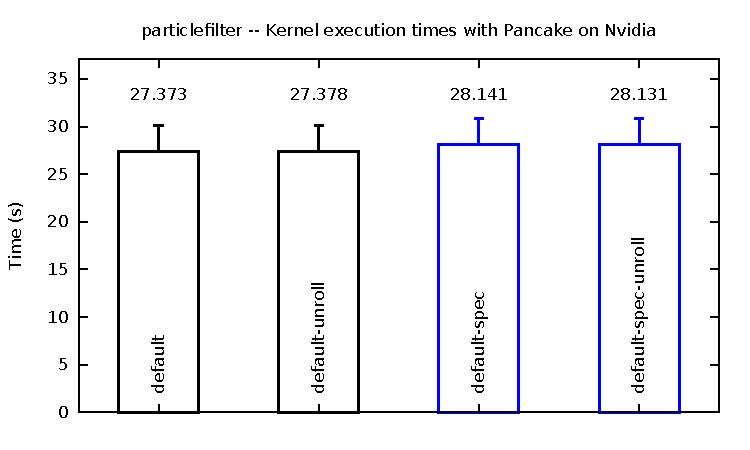
\includegraphics[width=3.0in]{charts/nvidia/particlefilter-exec}
\end{subfigure}}

\caption{\label{pancake-nvidia-table} Benchmark Timings for Pancake on Nvidia GTX 650 Ti}
\end{figure*}

%\restoregeometry



\section{Test Cases}
\label{test-cases}

Both implementations of Specialization Annotated OpenCL were tested with eight
test cases. Two of these test cases are newly written, while the other six were
taken from existing OpenCL benchmarks and vendor sample code and modified to
add specialization annotations.

\needspace{5\baselineskip}
\subsection{Newly Written Test Cases}

These programs were written specifically as test cases for this project. They
are intentionally written as naive implementations of the algorithm, without
any hand optimization. This may make performance effects from optimization
easier to see compared to the highly optimized test programs taken from
hardware benchmark suites.

\needspace{5\baselineskip}
\subsubsection{Gaussian Blur (blur)}

This program applies Gaussian blur to a large (5184x3456) greyscale image.
Because a 2D Gaussian blur can be calculated by applying two orthogonal 1D
Gaussian blurs to an image in sequence, this program runs two OpenCL kernels:
one to blur vertically and one to blur horizontally.

The kernels are each specialized on three arguments, the width and height of
the image and the radius of the blur effect. The radius is used for the inner
count of a tight inner loop, so its specialization was expected to result in a
measurable performance benefit due to unrolling.

With Specializing POCL, this test case saw a speedup at any optimization level,
but strangely ran slower at higher optimization levels than with no
optimization. Similarly, with Pancake there was a speedup on both graphics
cards, although the effect was much smaller on the Nvidia card.

\subsubsection{Matrix Multiply (mmul)}

This program multiplies two square matrices. Although matrix multiply programs
are common in OpenCL vendor samples, they are generally optimized to take
advantages of features like vector types. This program was written specifically
to be a simple and easily readable version of parallel matrix multiply.

The kernel is specialized on two arguments: the width and height of the
matrices. Since the iteration count of the inner loop is dependent on the width
and height of the matrices, this test was expected to show measurable
performance improvement from specialization.

With Specializing POCL, this test case showed a speedup of over 100\% from
specialization and unrolling, but the benefit was lost with a full set of
optimizations. With Pancake, it showed a speedup on both graphics cards. On the
AMD card, unrolling provided a significant performance increase while on the
Nvidia card it caused a slowdown compared to specialization without unrolling.

\needspace{5\baselineskip}
\subsection{SNU Port of NAS Parallel Benchmarks}

This is a port of the NASA Advanced Supercomputing Division's NAS Parallel
Benchmarksuite for large parallel HPC installations to OpenCL, performed by the
Center for Manycore Programming at Seoul National University in Korea
\cite{Van:2002:NAS}\cite{Seo:2011:NASPerf}.

These benchmarks are reasonably complex and require a significant amount of
communication in patterns that are not easily implemented in OpenCL, so the SNU
developers put significant effort into splitting kernels for synchronization
and hand optimizing to get high speedups. Further, many of the values that
would be the best candidates for specialization were already included in the
code as constants in order to get the best benchmark results. 

\subsubsection{Conjugate Gradient (nas-cg)}

This program is described by the NAS benchmark description as ``Solving an
unstructured sparse linear system by the conjugate gradient method'' with the
benchmark goal of testing ``irregular memory access and communication''.

For the OpenCL implementation this program was split into 13 kernels. The
kernels were all specialized on a single argument, {\tt n}, which remains
constant across any single execution of the program. As this argument is not
used directly as the bound of any loop, specialization and loop unrolling were
not expected to provide any performance benefit.

With Specializing POCL, this program showed a slowdown from specialization. On
Pancake it showed no benefit with either GPU.

\subsubsection{Scalar Penta-Diagonal (nas-sp)}

This program is intended to represent a larger HPC application that involves
multi-step processing of data. It performs a fluid dynamics simulation.

This program uses 26 OpenCL kernels. Fourteen of these kernels are specialized
on parameters that stay nearly constant in a single execution of the program,
some of which are used as loop bounds. This program was too complicated to
predict a result.

With Specializing POCL, this program surprisingly showed a large benefit from
specialization across all optimization levels. On Pancake, it showed no benefit
with either GPU.

\subsection{Nvidia OpenCL Samples}

These program were released by Nvidia as sample programs to demonstrate the
usage of their OpenCL implementation. They are written primarily for clarity to
serve as good examples, but include some features intended to improve
performance.

\subsubsection{Black-Scholes Option Pricing (nv-bs)}

According to Nvidia, ``This sample evaluates fair call and put prices for a
given set of European options by the Black-Scholes formula.'' 

This kernel is specialized on a single variable, {\tt OptN}, which is the maximum
number of iterations of the algorithm. This is a constant across multiple calls
to the kernel in the test program. It specifies the iteration limit of a
reasonably tight inner loop, but the loop start varies across work items so the
loop may not be possible to unroll.

With Specializing POCL, this program showed a slight slowdown from
specialization. On Pancake, it showed a slight speedup with unrolling on AMD,
while on Nvidia specialization caused a slowdown with unrolling enabled.

\subsubsection{DCT (nv-dct)}

This program performs a Discrete Cosine Transform on an image.

The kernel is specialized on the stride, width, and height of the input image,
and the block size of the transform, which all remain constant in the test
program. The program was initially developed with a constant block size of
eight, but this was made a variable in order to exercise specialization. Since
all the loops in the program are a number of iterations equal to the block size,
this program was expected to see speedups due to specialization.

With Specializing POCL, this program showed a significant speedup from
specialization in combination with either loop unrolling or a full set of
optimizations. On Pancake, it showed a slight speedup with AMD and no effect on
Nvidia.

\subsection{Rodinia Benchmarks}

These benchmarks were found in the Rodinia Benchmark
Suite\footnote{\url{https://www.cs.virginia.edu/~skadron/wiki/rodinia}}, from
the University of Virginia. This suite is intended to compare the performance
of hardware and OpenCL implementations. The benchmarks are extracted from real
world scientific computing applications, and are heavily hand optimized for
performance including some hard-coded constants.

\subsubsection{Mandelbrot (mandelbrot)}

This generates a 2048x2048 image of the Mandelbrot set. It has a single OpenCL
kernel to generate this image.

The kernel is specialized on four arguments: the width and height of the image,
the zoom level, and the maximum number of iterations of the tight inner loop.
Although the number of iterations of the tight inner loop is bounded by a
specialized argument, each instance of the kernel may iterate fewer times. The
outcome for this benchmark was hard to predict due to the loop structure.

With Specializing POCL, this benchmark showed no speedup from specialization.
On Pancake, it showed a significant speedup on AMD and a small speedup on
Nvidia.

\subsubsection{Particle Filter (particlefilter)}

This program tries to estimate current location based on a model of movement
and fuzzy location measurements. 

The main kernel is specialized on the number of particles used, which is
constant through an execution of the program. This kernel has a loop based on
the number of particles, but the start point is based on the current particle
so the loop may not be possible to unroll. Again, this loop structure is
difficult to make predictions about.

With both Specializing POCL and Pancake, this benchmark showed no speedup from
specialization.

\section{Conclusion and Future Work}

Specialization Annotated OpenCL is a promising technique for speeding up OpenCL
programs. It showed speedups on many of the test cases, and since it must be
explicitly enabled by an annotation, can simply be left disabled in cases where
it may cause a slowdown.

It is our hope that specialization will be considered for future programming
systems based on JIT compilation as an optional optimization. With additional
work on automatically determining specialization variables, it would be a
useful general addition to the JIT compilation capability of LLVM.

\balancecolumns

Specialization seems to provide better performance benefits for graphics
processors than it does for CPUs, so future work on Specialization Annotated
OpenCL will focus on open source OpenCL runtimes like Clover (for AMD GPUs) and
Beignet (for Intel GPUs). When this work was done, neither runtime was stable
enough for general use, but that situation is quickly improving.

Another avenue for future work would be to automatically select specialization
parameters rather than requiring programmer annotations. It is not obvious what
the best way to do this is. It may require speculative specialization and
profiling, which would be relatively expensive. But if it could be made to work
effectively it would make specialization a transparent optimization suitable for
use in JIT-based programming systems.

Both Specializing POCL and Pancake are available under open source licenses,
although at the time of this writing neither is sufficiently polished for
general use.

\begin{itemize}
    \item \url{https://github.com/NatTuck/pocl}
    \item \url{https://github.com/NatTuck/pancake}
\end{itemize}

\bibliographystyle{abbrv}
\bibliography{references}


\end{document}
